% !TEX TS-program = pdflatex
% !TEX encoding = UTF-8 Unicode

\documentclass{beamer}
% for handouts: \documentclass[handout]{beamer}

%\setbeamertemplate{background canvas}[vertical shading][bottom=white,top=structure.fg!25]
% or whatever

\usetheme[compress]{Amsterdam}
%\setbeamertemplate{headline}{}
%\setbeamertemplate{footline}{}
%\setbeamersize{text margin left=0.5cm}
  
\usepackage[english]{babel}
\usepackage{listings}
\usepackage{geometry}
\usepackage{hyperref}

\usepackage{color}
\usepackage[T1]{fontenc}
\usepackage[utf8]{inputenc}
\usepackage{lmodern}

\usepackage{multicol}
\lstset{
basicstyle=\scriptsize\ttfamily,
columns=flexible,
breaklines=true,
numbers=left,
%stepsize=1,
numberstyle=\tiny,
backgroundcolor=\color[rgb]{0.85,0.90,1}
}


\begin{document}

\title[Big Data and Automated Content Analysis]{\textbf{Big Data and Automated Content Analysis I+II} \\ Week 4 -- Wednesday \\ Sentiment Analysis}
\author[Damian Trilling]{Damian Trilling \\ ~ \\ \footnotesize{d.c.trilling@uva.nl \\@damian0604} \\ \url{www.damiantrilling.net}}
\date{26 February 2020}
\institute[UvA]{Afdeling Communicatiewetenschap \\Universiteit van Amsterdam}


\begin{frame}{}
\titlepage
\end{frame}

\begin{frame}{Today}
\tableofcontents
\end{frame}



\section{Different types of analysis}

\begin{frame}{What we already can do}
\begin{block}{with regard to data collection:}<1->
\begin{itemize}
\item query a (JSON-based) API (GoogleBooks, Twitter)
\item handle CSV files
\item handle JSON files 
\end{itemize}
\end{block}

\begin{block}{with regard to analysis:}<2->
Not much. We counted some frequencies and calculated some averages.
\end{block}

\end{frame}



\subsection{What can we do?}
\begin{frame}
Data analysis: Overview\\
What can we do? \\ ~\\
\onslide<2>{\textbf{What do you think? What are interesting methods to analyze large data sets (like, e.g., social media data? What questions can they answer?)}}
\end{frame}

\begin{frame}{What else can we do?}
\begin{block}{For example}
\begin{itemize}
\item sentiment analysis
\item automated coding with regular expressions
\item natural language processing
\item supervised and unsupervised machine learning
\item network analysis
\end{itemize}
\end{block}
\end{frame}

\begin{frame}{What else can we do?}
\begin{block}{Or ideally\ldots}
\ldots a combination of these techniques.
\end{block}
\end{frame}





\subsection{Systematizing analytical approaches}
\begin{frame}
\textbf{Overview}\\
Systematizing analytical approaches
\end{frame}

\begin{frame}{Systematizing analytical approaches}
Taking the example of Twitter:
\begin{block}{Analyzing the \emph{structure}}
\begin{itemize}
\item Number of Tweets over time
\item singleton/retweet ratio
\item Distribution of number of Tweets per user
\item Interaction networks
\end{itemize}
\end{block}
\onslide<2->{
{\textbf{$\Rightarrow$ Focus on the amount of content and on the question who interacts with whom, not on what is said}}\\~\\ }
{\tiny Bruns, A., \& Stieglitz, S. (2013). Toward more systematic Twitter analysis: metrics for tweeting activities. \emph{International Journal of Social Research Methodology}. doi:10.1080/13645579.2012.756095\\ }
\end{frame}

\begin{frame}{Systematizing analytical approaches}
Taking the example of Twitter:
\begin{block}{Analyzing the \emph{content}}
\begin{itemize}
\item Sentiment analysis
\item Word frequencies, searchstrings
\item Co-word analysis ($\Rightarrow$frames)
\end{itemize}
\end{block}
\onslide<2->{
{\textbf{$\Rightarrow$ Focus on what is said}}}
\end{frame}

\begin{frame}{Systematizing analytical approaches}

{\textbf{$\Rightarrow$ It depends on your reserach question which approach is more interesting!}}
\end{frame}






\begin{frame}{Automated Content Analysis}
	\makebox[\columnwidth]{
		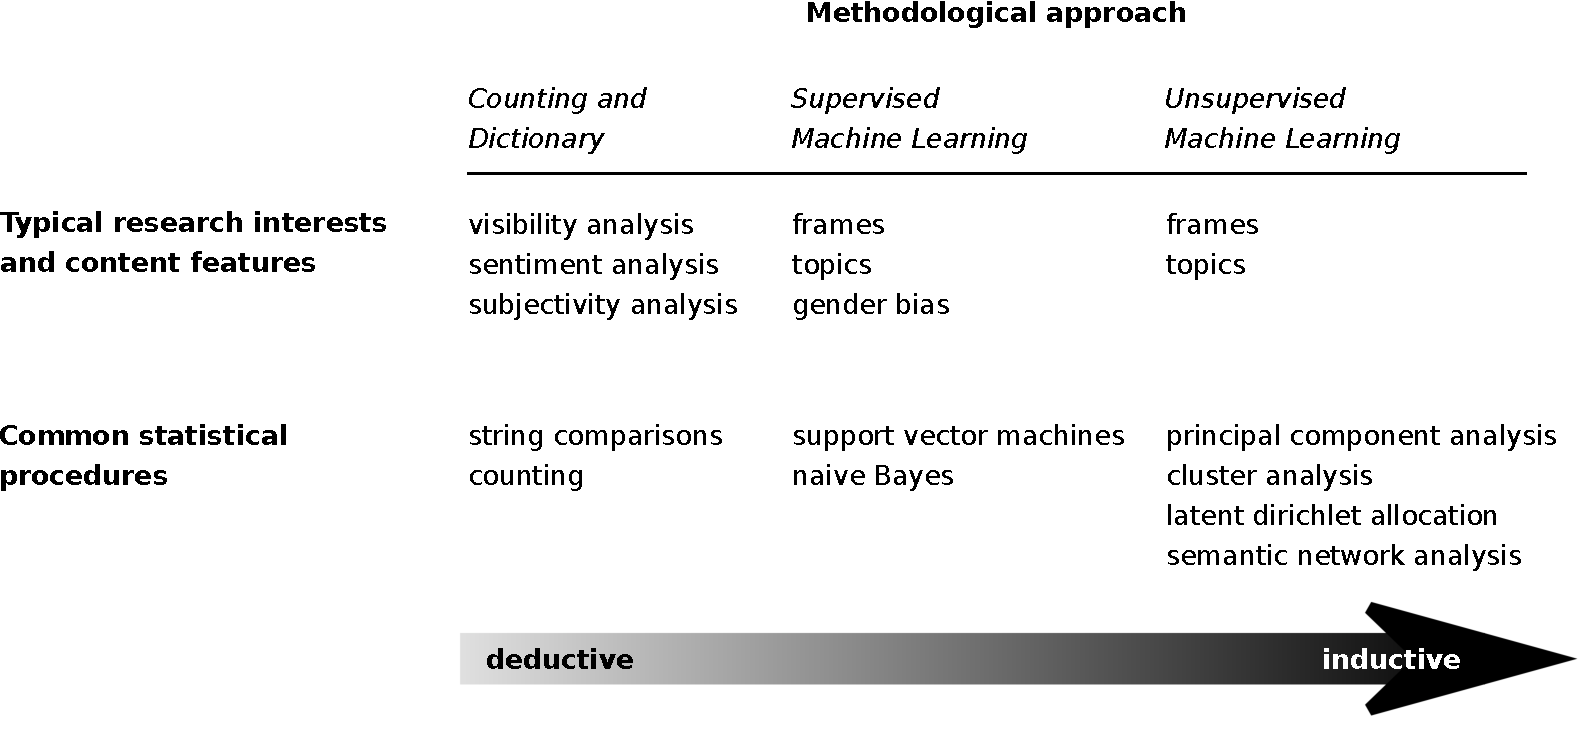
\includegraphics[width=\columnwidth,height=\paperheight,keepaspectratio]{../../pictures/boumanstrilling2016}}
	\\
	\tiny
	Boumans, J.W., \& Trilling, D. (2016). Taking stock of the toolkit: An overview of relevant automated content analysis approaches and techniques for digital journalism scholars. \emph{Digital Journalism, 4}, 1. 8--23.
\end{frame}






\section[Sentiment analysis]{Data analysis 1: Sentiment analysis}
\subsection{What is it?}
\begin{frame}
Data analysis 1:\\
\textbf{Sentiment analysis}
\end{frame}


\begin{frame}{What is sentiment analysis?}
\begin{block}{Extracting subjective information from texts}
\begin{itemize}
\item<2->  the author's attitude towards the topic of the text
\item<3-> \emph{polarity}: negative---positive
\item<4-> \emph{subjectivity}: neutral---subjective *
\item<5-> advanced approaches: different emotions
\end{itemize}
~\\ 
\footnotesize{
\onslide<6->{* Less sophisticated approaches do not see this as a sperate dimension but simply calculate $objectivity=1-(negativity+positivity)$}}
\end{block}
\end{frame}



\begin{frame}{Applications}
\begin{block}{Who uses it?}
\begin{itemize}
\item Companies
\item especially for Web Analytics
\item Social Scientists
\item applications in data journalism, politics, \ldots
\end{itemize}
Many references to examples in Mostafa (2013).
\end{block}
~\\
$\Rightarrow$ Cases in which you have a huge amount of data or real-time data and you want to get an idea of the tone. \\ ~
\par
\tiny{Mostafa, M. M. (2013). More than words: Social networks’ text mining for consumer brand sentiments. \emph{Expert Systems with Applications, 40}(10), 4241– 4251. doi:10.1016/j.eswa.2013.01.019}\\
\end{frame}


\begin{frame}[fragile]{Example}
\begin{lstlisting}
>>> sentiment("Great service by @NSHighspeed")
(0.8, 0.75)
>>> sentiment("Bad  service by @NSHighspeed")
(-0.6166666666666667, 0.6666666666666666)
\end{lstlisting}
~\\
\footnotesize{(polarity, subjectivity) with \\ ~ \\
 $-1 \leq polarity \leq +1$\\
 $0 \leq subjectivity \leq +1$ )} \\~\\
\vskip 1cm 
\tiny{This is the module pattern.nl \\ De Smedt, T., \& Daelemans W. (2012).  Pattern for Python. \emph{Journal of Machine Learning Research, 13}, 2063-2067.\\}
\end{frame}

\subsection{Bag-of-words approaches}
\begin{frame}
Data analysis 1: Sentiment analysis\\
Bag-of-words approaches
\end{frame}


\begin{frame}{Bag-of-words approaches}
\begin{block}{How does it work?}
\begin{itemize}
\item We take each word of a text and look if it's positive or negative.
\begin{itemize}
\item<2-> Most simple way: compare it with a list of negative words and with a list of positive words {\small(That's what Mostafa (2013) did)}
\item<3-> More advanced: look up a subjectivity score from a table 
\end{itemize}
\item<4-> e.g., add up the scores and average them.
\end{itemize}
\end{block}
\end{frame}


\begin{frame}[fragile]{How to do this}
If you were to run an analyis like the one by Mostafa (2013), how could you do this?
\end{frame}

\begin{frame}[fragile]{How to do this}
\scriptsize{ 
(given a \emph{string} \texttt{tekst} that you want to analyze and two 
\emph{lists} of strings with negative and positive words, 
\texttt{lijstpos=$[$"great","fantastic",\ldots,"perfect"$]$} and \texttt{lijstneg})\\
}

\begin{lstlisting}
sentiment=0
for woord in tekst.split():
    if woord in lijstpos:
        sentiment=sentiment+1    #same as sentiment+=1
    elif woord in lijstneg:
        sentiment=sentiment-1    #same as sentiment-=1
print (sentiment)
\end{lstlisting}
%if sentiment > 0:
%    print "This was a positive text".
%elif sentiment < 0:
%    print "This was a negative text".    
%elif sentiment == 0:
%    print "We could not identify any tendency".    
\end{frame}


\begin{frame}[fragile]{Do we need to have the lists in our program itself?}
No.\\
You could have them in a separate text file, one per row, and then read that file directly to a list.\\
\begin{lstlisting}
poslijst=open("filewithonepositivewordperline.txt").read().splitlines()
neglijst=open("filewithonenegativewordperline.txt").read().splitlines()
\end{lstlisting}
\end{frame}


{\setbeamercolor{background canvas}{bg=black}
\begin{frame}[plain]
\makebox[\linewidth]{
\includegraphics[width=\paperwidth,height=\paperheight,keepaspectratio]{../../pictures/woordenlijst1.png}}
\end{frame}
}


\begin{frame}{More advanced versions}
\begin{itemize}
\item CSV files or similar tables with weights
\item Or some kind of dict?
\end{itemize}
\end{frame}

{\setbeamercolor{background canvas}{bg=black}
\begin{frame}[plain]
\makebox[\linewidth]{
\includegraphics[width=\paperwidth,height=\paperheight,keepaspectratio]{../../pictures/woordenlijst2.png}}
\end{frame}
\begin{frame}[plain]
\makebox[\linewidth]{
\includegraphics[width=\paperwidth,height=\paperheight,keepaspectratio]{../../pictures/woordenlijst3.png}}
\end{frame}
}



\begin{frame}{Mustafa 2013: Interpreting the output}

\begin{columns}
\column{.7\textwidth}
\makebox[\columnwidth]{
\includegraphics[width=\paperwidth,height=.7\paperheight,keepaspectratio]{../../pictures/plaatje_uit_mostafa2013.png}
}
\column{.3\textwidth}
\onslide<2->{Your thoughts?}
\onslide<3->{
\begin{itemize}
\item each word counts equally (1)
\item many tweets contain no words from the list. What does this mean?
\item Ways to improve BOW approaches?
\end{itemize}
}
\end{columns}
\end{frame}

% nog iets met die scores. dus een beter voorbeeld. Een tweede


\begin{frame}{Bag-of-words approaches}
\begin{block}{pro}<2->
\begin{itemize}
\item easy to implement
\item easy to modify:
\begin{itemize}
\item add or remove words
\item make new lists for other languages, other categories (than positive/negative), \dots
\end{itemize}
\item easy to understand (transparency, reproducability)
\end{itemize}
\end{block}
\par
\tiny{e.g., Schut, L. (2013). Verenigde Staten vs. Verenigd Koningrijk: Een automatische inhoudsanalyse naar verklarende factoren voor het gebruik van positive campaigning en negative campaigning door vooraanstaande politici en politieke partijen op Twitter. \emph{Bachelor Thesis}, Universiteit van Amsterdam.}\\
\end{frame}



\begin{frame}{Bag-of-words approaches}
\begin{block}{con}
\begin{itemize}
\item simplistic assumptions
\item e.g., intensifiers cannot be interpreted ("really" in "really good" or "really bad")
\item or, even more important, negations.
\end{itemize}
\end{block}
\end{frame}



\subsection{Advanced approaches}
\begin{frame}
Data analysis 1: Sentiment analysis\\
Advanced approaches
\end{frame}


\begin{frame}{Improving the BOW approach}
\begin{block}{Example: The Sentistrenght algorithm}
\begin{itemize}
\item $-5\ldots-1$ and $+1\ldots+5$
\item spelling correction
\item "booster word list" for strengthening/weakening the effect of the following word
\item interpreting repeated letters ("baaaaaad"), CAPITALS and !!!
\item idioms
\item negation 
\item ldots
\end{itemize}
\end{block}
~ \\
\tiny{Thelwall, M., Buckley, K., \& Paltoglou, G. (2012). Sentiment strength detection for the social Web. \emph{Journal of the American Society for Information Science and Technology, 63}(1), 163-173.\\}
\end{frame}


\begin{frame}{Advanced approaches}
\begin{block}{Take the structure of a text into account}
\begin{itemize}
\item Try to apply linguistics concepts to identify sentence structure
\item can identify negations
\item can interpret intensifiers
\end{itemize}
\end{block}
\end{frame}


\begin{frame}[fragile]{Example}
\begin{lstlisting}
from pattern.nl import sentiment
>>> sentiment("Great service by @NSHighspeed")
(0.8, 0.75)
>>> sentiment("Really")
(0.0, 1.0)
>>> sentiment("Really Great service by @NSHighspeed")
(1.0, 1.0)
\end{lstlisting}
~\\
\footnotesize{(polarity, subjectivity) with \\
 $-1 \leq polarity \leq +1$\\
 $0 \leq subjectivity \leq +1$ )\\} ~ \\
Unlike in pure bag-of-words approaches, here, the overall sentiment is not just the sum or the average of its parts! \\
\tiny{De Smedt, T., \& Daelemans W. (2012).  Pattern for Python. \emph{Journal of Machine Learning Research, 13}, 2063-2067.}
\end{frame}




\begin{frame}{Advanced approaches}
\begin{block}{pro}<2->
\begin{itemize}
\item understand intensifiers or negation
\item thus: higher accuracy
\end{itemize}
\end{block}
\begin{block}{con}<3->
\begin{itemize}
\item Black box? Or do we understand the algorithm?
\item Difficult to adapt to own needs
\item \emph{really} much better results?
\end{itemize}
\end{block}
\end{frame}



\subsection{A sentiment analysis tailored to your needs!}
\begin{frame}
Data analysis 1: Sentiment analysis\\
A sentiment analysis tailored to your needs!
\end{frame}




\begin{frame}{A sentiment analysis tailored to your needs!}
\begin{block}{Identifying suicidal texts}
\begin{itemize}
\item Bag-of-words-approach with very specific dictionary
\item added negation
\item added regular expression search for key phrases
\item Very specific design requirements: False positives are OK, false negatives not!
\end{itemize}
\end{block}
\par
\tiny{Huang, Y.-P., Goh, T., \& Liew, C.L. (2007). Hunting suicide notes in web 2.0 – preliminary findings. \emph{Ninth IEEE International Symposium on Multimedia}. Retrieved from http://ieeexplore.ieee.org/stamp/stamp.jsp?tp=\&arnumber=4476021}\\
\end{frame}

\begin{frame}{}
Already this still relatively simple approach seems to work satisfactory, but if 106 scientists from 24 competing teams (!) work on it, they can 
\begin{block}{group suidide notes by these characteristics:}<2->
\begin{multicols}{2}
{\small {
\begin{itemize}
\item swear
\item family
\item friend
\item positive emotion
\item negative emotion
\item anxiety
\item anger
\item sad
\item cognitive process
\item biology
\item sexual
\item ingestion
\item religion
\item death
\end{itemize}
}}
\end{multicols}
\end{block}
\par
\tiny{Pestian, J.P.; Matykiewicz, P., Linn-Gust, M., South, B., Uzuner, O., Wiebe, J., Cohen, K.B., Hurdle, J., \& Brew, C. (2012). Sentiment analysis of suicide notes: A shared task. \emph{Biomedical Informatics Insights, 5}(1), p. 3-16. Retrieved from http://europepmc.org/articles/PMC3299408?pdf=render}\\
\end{frame}



\subsection{Packages for sentiment analysis}

\begin{frame}[plain]
Packages for sentiment analysis
\end{frame}


\begin{frame}{Which packages are easy to use?}
	
\begin{description}
	\item[vader]<1-> pro: in NLTK module, con: English only
	\item[pattern]<2-> pro: mutiple languages (including Dutch)
	\item[sentistrength]<3-> pro: multiple languages, widely used, con: needs Python wrapper, license
	
\end{description}

\onslide<3->{
{\tiny{vader: Chapter 6.3; pattern: Chapter 6.5; sentistrength: Chapter 6.4}}}


\onslide<4>{\textbf{BUT: Keep in mind that the results of \emph{any} off-the-shelf-package might be biased and/or noisy in \emph{your} domain!}	}

\end{frame}


\begin{frame}%{Agreement between off-the-shelf packages}
	\makebox[\columnwidth]{
	\includegraphics[width=\columnwidth,height=.8\paperheight,keepaspectratio]{../../pictures/boukessentiment}}
\\
\tiny
Boukes, M., van der Velde, R.N., \& Vliegenthart, R. (2018). The good and bad in economic news: Comparing (automatic) measurements of sentiment in Dutch economic news. \emph{International Communication Association conference}, Prague, Czech Republic.
\end{frame}


\begin{frame}%{Agreement between off-the-shelf packages}
	\makebox[\columnwidth]{
		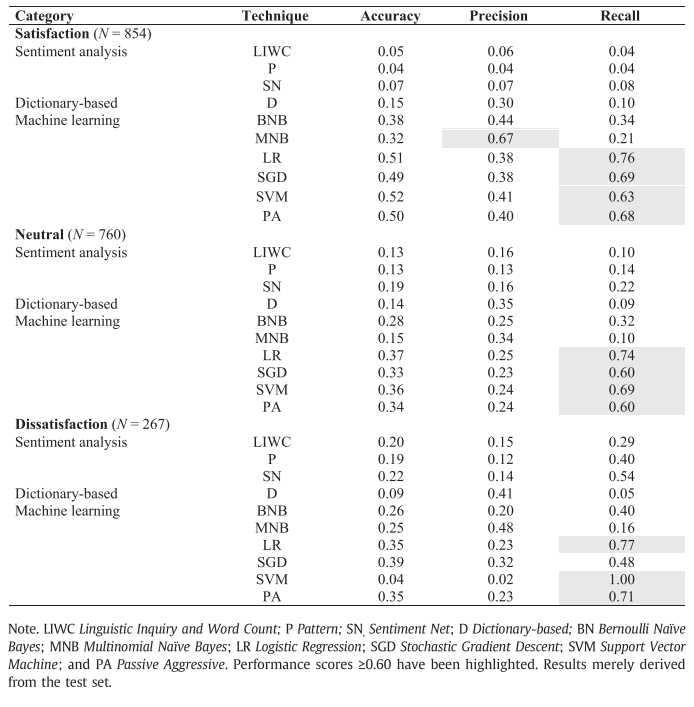
\includegraphics[width=\columnwidth,height=.8\paperheight,keepaspectratio]{../../pictures/vermeer2019}}
	\\
	\tiny
Vermeer, S. A. M., Araujo, T., Bernritter, S. F., \& van Noort, G. (2019). Seeing the wood for the trees: How machine learning can help firms in identifying relevant electronic word-of-mouth in social media. International Journal of Research in Marketing, 36(3), 492–508. doi:10.1016/j.ijresmar.2019.01.010
\end{frame}



\subsection{A receipe}

\begin{frame}{A possible receipe for doing your sentiment analysis}
	
\begin{enumerate}
	\item Construct a list \texttt{data} of strings with your input data
	\item Create an empty list \texttt{sent} for storing the results
	\item For each text \texttt{t} in \texttt{data}, estimate the sentiment of \texttt{t} and append the result to \texttt{sent}\footnote{use multiple lists instead if you estimate for instance subjectivity \emph{and} polarity}
	\item Confirm that \texttt{len(data) == len(sent)}
	\item use \texttt{zip()} and a  \texttt{csv.writer} to write input and output next to each other to a csv file.
\end{enumerate}

\end{frame}



\subsection{Machine Learning as alternative}
\begin{frame}{Superivsed ML ($\Rightarrow$ week 9)}
	An alternative state-of-the-art approach:
	\begin{block}{Use supervised machine learning}
		\begin{itemize}
			\item Instead of defining rules, hand-code (``annotate'') the sentiment of some tweets manually and let the computer find out which words or characters (``features'') predict sentiment
			\item Then use this model to predict sentiment for other tweets
			\item Essentially the same like what you know since the second year of your Bachelor: regression analysis (but now with DV sentiment and IV's word occurrences)
			% \item $\Rightarrow$ week 7
		\end{itemize}
		\tiny{Gonzalez-Bailon, S., \& Paltoglou, G. (2015). Signals of public opinion in online communication: A comparison of methods and data sources. \emph{The ANNALS of the American Academy of Political and Social Science, 659}(1), 95-–107.}
	\end{block}
	
\end{frame}


%
%
%\section[Stopword removal]{NLP-preview: Stopword removal}
%\begin{frame}
%Natural Language Processing preview:\\
%\textbf{Stopword removal} \\
%\vspace{1cm}
%\onslide<2>{Why now? --- Because the logic of the algorithm is very much related to the one of our first simple sentiment analysis}
%\end{frame}
%
%\subsection{Natural language processing}
%\begin{frame}{Stopword removal: What and why?}
%\begin{block}{Why remove stopwords?}
%\begin{itemize}
%\item If we want to identify key terms (e.g., by means of a word count), we are not interested in them
%\item If we want to calculate document similarity, it might be inflated
%\item If we want to make a word co-occurance graph, irrelevant information will dominate the picture
%\end{itemize}
%\end{block}
%\end{frame}
%
%\subsection{A simple algorithm}
%\begin{frame}[fragile]{Stopword removal: How}
%\begin{lstlisting}
%testo='He gives her a beer and a cigarette.'
%testonuovo=""
%stopwords=['and','the','a','or','he','she','him','her']
%for verbo in testo.split():
%    if verbo not in stopwords:
%       testonuovo=testonuovo+verbo+" "
%\end{lstlisting}
%What do we get if we do:
%\begin{lstlisting}
%print (testonuovo)
%\end{lstlisting}
%Can you explain the algorithm?
%\end{frame}
%
%\begin{frame}[fragile]{We get:}
%\begin{lstlisting}
%>>> print  (testonuovo)
%'He gives beer cigarette. '
%\end{lstlisting}
%Why is "He" still in there? \\ How can we fix this?
%\end{frame}
%
%\begin{frame}[fragile]{Stopword removal}
%\begin{lstlisting}
%testo='He gives her a beer and a cigarette.'
%testonuovo=""
%stopwords=['and','the','a','or','he','she','him','her']
%for verbo in testo.split():
%    if verbo.lower() not in stopwords:
%       testonuovo=testonuovo+verbo+" "
%\end{lstlisting}
%\end{frame}
%
%
%




\section[Next meetings]{Take-home message, next meetings, \& exam}
\begin{frame}
Take-home message\\
Mid-term take-home exam\\
Next meetings
\end{frame}



\begin{frame}{Take-home messages}
\begin{block}{What you should be familiar with:}
\begin{itemize}
\item You should have \emph{completely} understood last week's exercise. Re-read it if neccessary.
\item Approaches to the analysis (e.g., structure vs. content)
\item Types of sentiment analysis, application areas, pros and cons
\end{itemize}
\end{block}
\end{frame}


\begin{frame}{Mid-term take home exam}
\begin{block}{Week 5: Friday, 6 March, to Tuesday, 10 March}
\begin{itemize}
\item You get the exam on Friday at the end of the meeting
\item Answers have to be handed in no later than Tuesday evening, 23.59
\item 20\% of final grade
\item 3 questions:
\begin{enumerate}
\item Literature question: E.g., different methods (``Explain how\ldots is done'') and/or epistemological or theoretical implications (``What does this mean for social-scientific research?'')
\item Empirical question (conceptual)
\item Empirical question (actual programming task)
\end{enumerate}
If you \emph{fully} understood all exercises until now, it shouldn't be difficult and won't take too long. But give yourself \emph{a lot} of buffer time!!! 
\end{itemize}
\end{block}
\end{frame}



\begin{frame}{Next meetings}
\begin{block}{Friday, 28--2}
Task for during the meeting: Conduct an own sentiment analysis!

You can bring your own data (you will probably learn more!), but then already think about how to write some script to read the data (as we did last week and as described in Chapter 5).
\end{block}

\end{frame}




\end{document}

